\documentclass[11pt,a4paper]{article}

\usepackage[margin=1in]{geometry}
\usepackage{graphicx}
\usepackage{amsmath}
\usepackage{amsfonts}
\usepackage{amssymb}
\usepackage{booktabs}
\usepackage[hyphens]{url}
\usepackage[hidelinks]{hyperref}
\usepackage{caption}
\usepackage{subcaption}
\usepackage{siunitx}
\usepackage{float}
\usepackage{authblk}
\usepackage{algorithm}
\usepackage{algorithmic}
\usepackage{xcolor}
\usepackage{enumitem}

\definecolor{adamwcolor}{HTML}{0000FF}
\definecolor{muoncolor}{HTML}{FF0000}

\title{\Large\bfseries Muon vs AdamW: Learning Rate And Scaling Small LLMs}

\author[1]{Vuk Rosić}
\author[2]{Claude}
\affil[1]{Óbuda University, \texttt{vukrosic1@gmail.com}}
\affil[2]{Anthropic}

\date{July 22, 2025}

\begin{document}
\maketitle

\begin{center}
\vspace{1em}
\noindent\textbf{Resources:} 
\href{https://github.com/vukrosic/muon-optimizer-research}{GitHub} \quad - \quad
\href{https://github.com/vukrosic/muon-optimizer-research/blob/main/muon_vs_adamw_for_llms.ipynb}{Jupyter Notebook}
\end{center}

\begin{abstract}
Optimizer selection critically impacts the training dynamics and final performance of large language models. While AdamW~\cite{loshchilov2017decoupled} remains the predominant choice, recent innovations like Muon~\cite{jordan2024muon}—which incorporates gradient orthogonalization via Newton-Schulz iteration—promise improved training stability and convergence. 

We present a systematic empirical comparison across four Transformer LLM sizes (11M to 108M parameters) trained on SmolLM-Corpus. Our study reveals a pronounced scale-dependent performance divergence: Muon~\cite{jordan2024muon} demonstrates modest improvements on smaller models but achieves dramatic superiority on larger architectures. Notably, on our 108M parameter model, Muon attains 94.6\% validation accuracy while AdamW fails catastrophically at 28.4\%—a 233\% relative improvement, showing that AdamW is a lot more sensitive to a suboptimal learning rate, while Muon tolerates larger range of learning rates.

Despite a 4-5\% computational overhead per training step, possibly because AdamW implementation by PyTorch is more optimized, Muon’s strong convergence and ability to scale well make it a promising alternative to AdamW, especially for training large language models. These results highlight how important it is to choose the right optimizer when working at scale, and suggest that techniques like gradient conditioning should be more widely used in large neural network training.
\end{abstract}

\begin{figure}[H]
    \centering
    \begin{subfigure}[b]{0.48\textwidth}
        \centering
        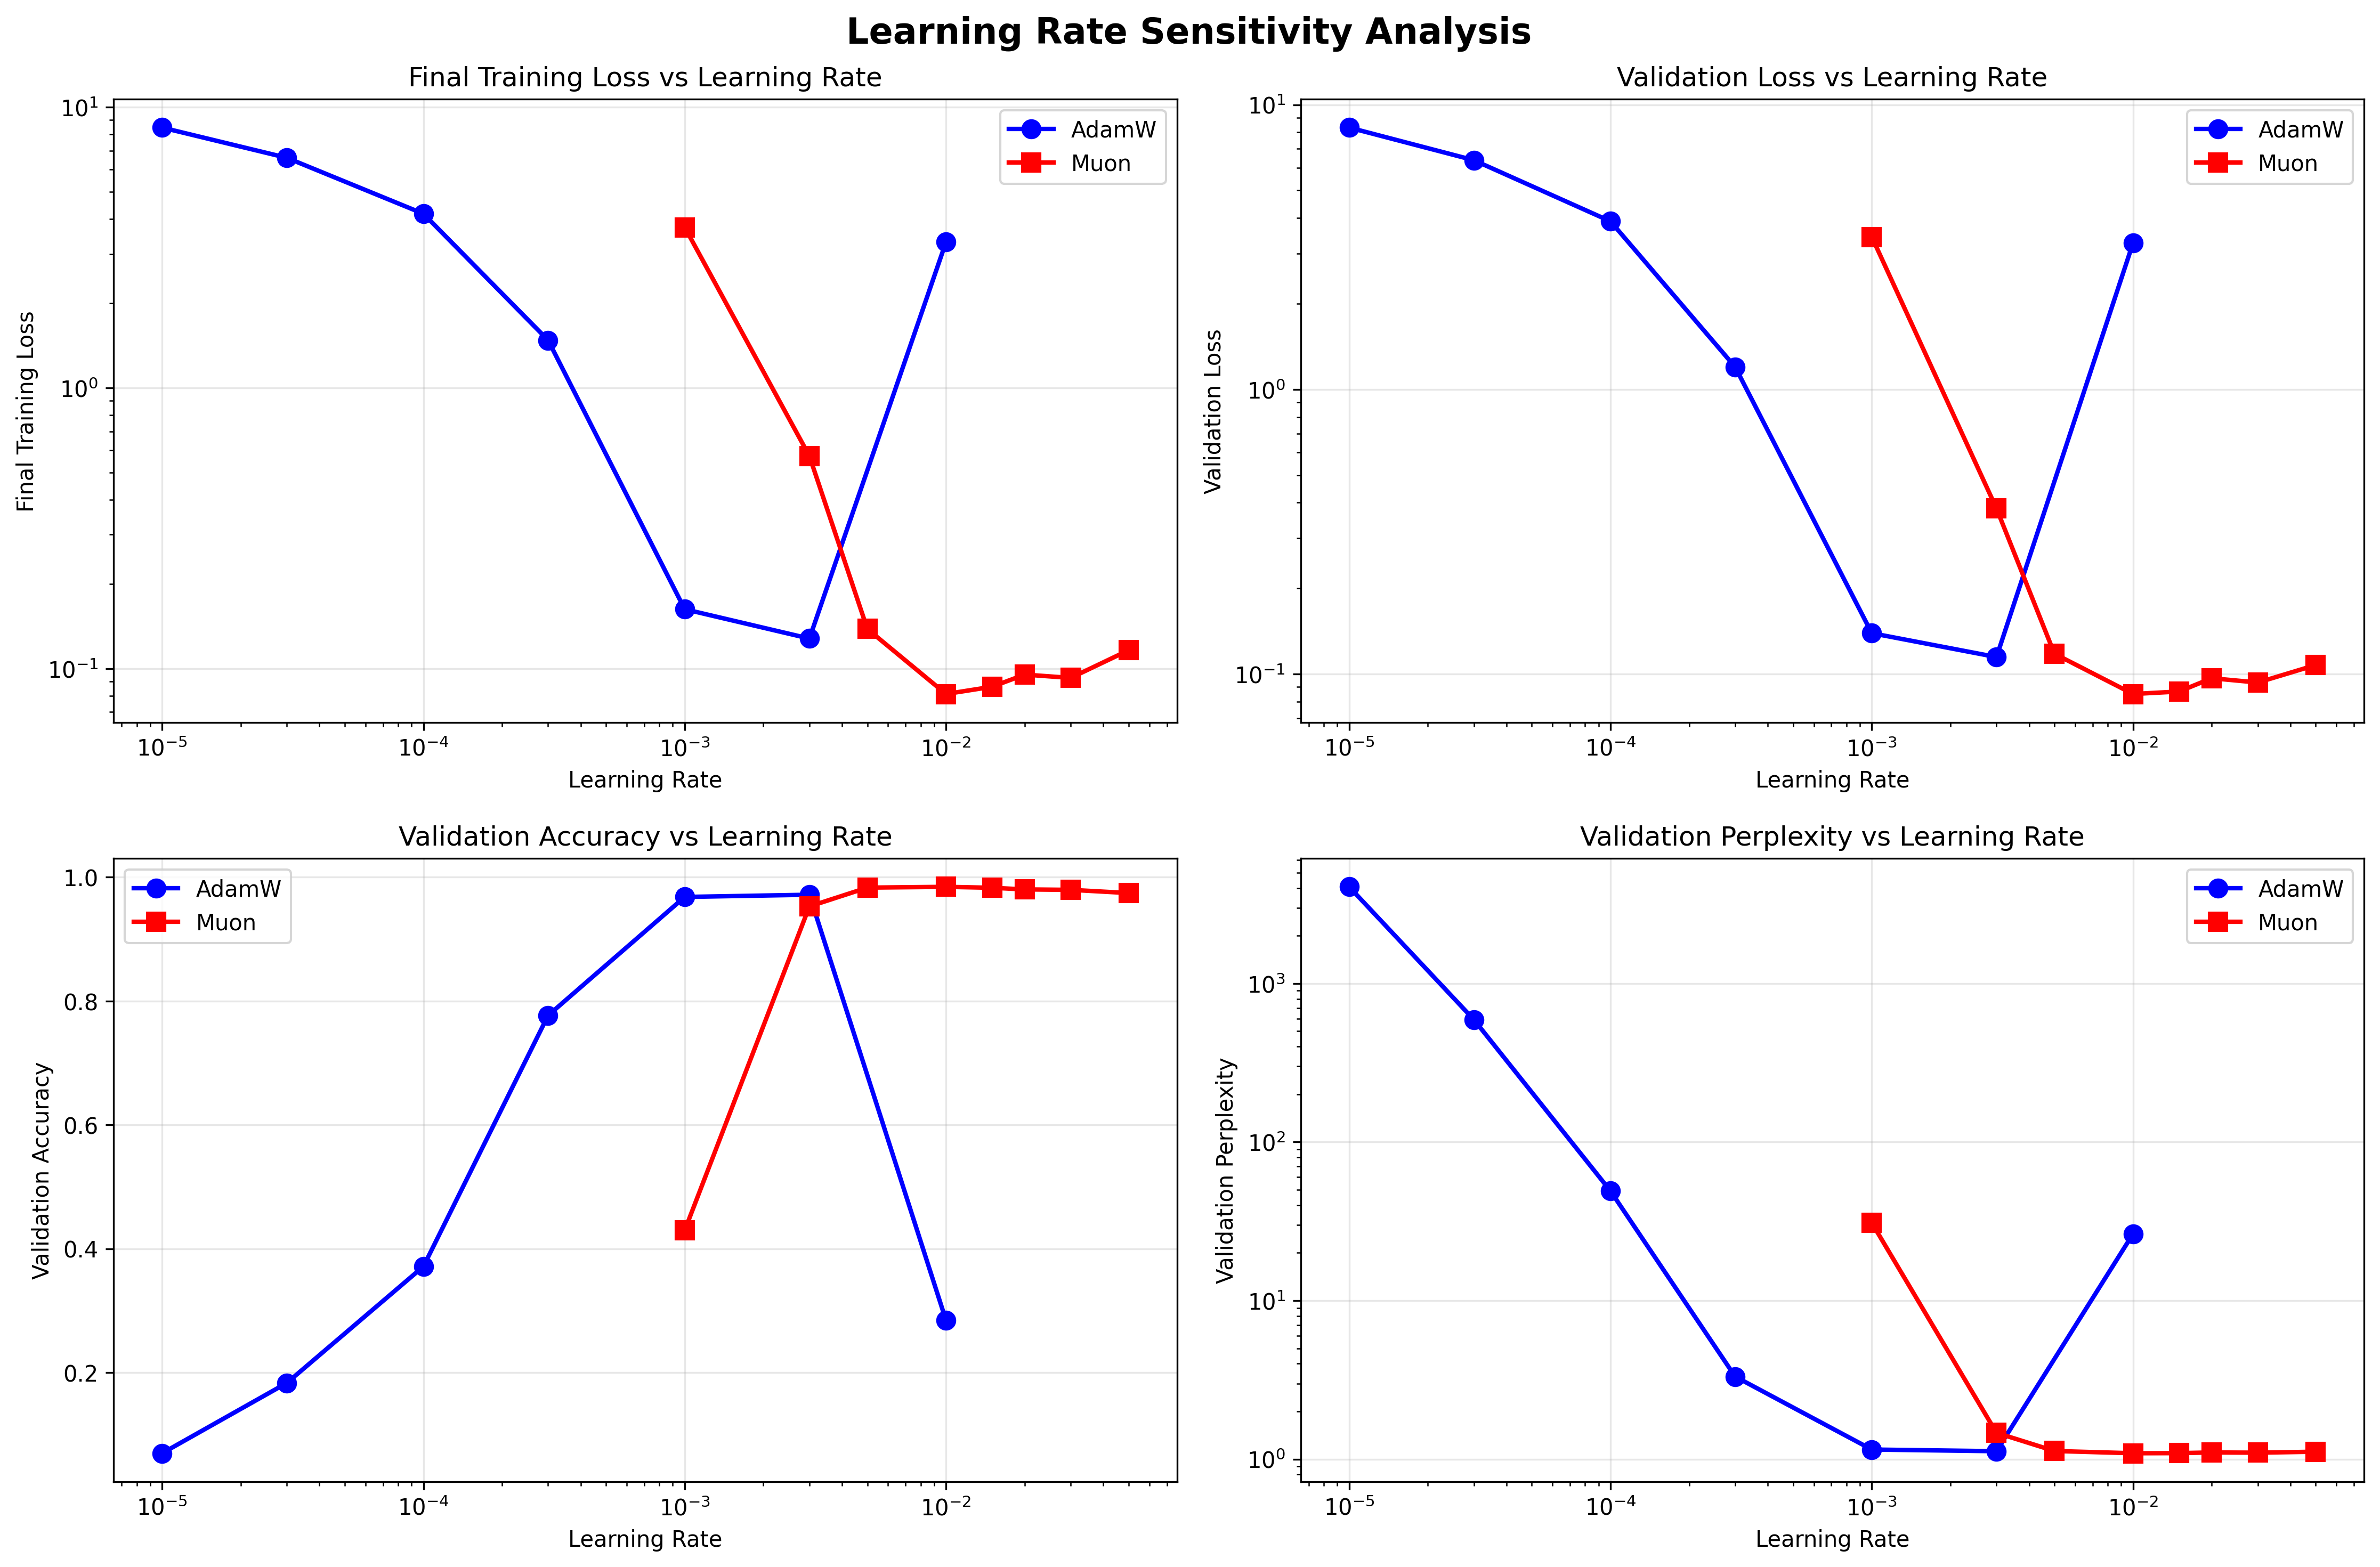
\includegraphics[width=\textwidth]{results/experiment_1_learning_rate/lr_sensitivity_analysis.png}
        \caption{Learning rate sensitivity comparison}
        \label{fig:preview_lr}
    \end{subfigure}
    \hfill
    \begin{subfigure}[b]{0.48\textwidth}
        \centering
        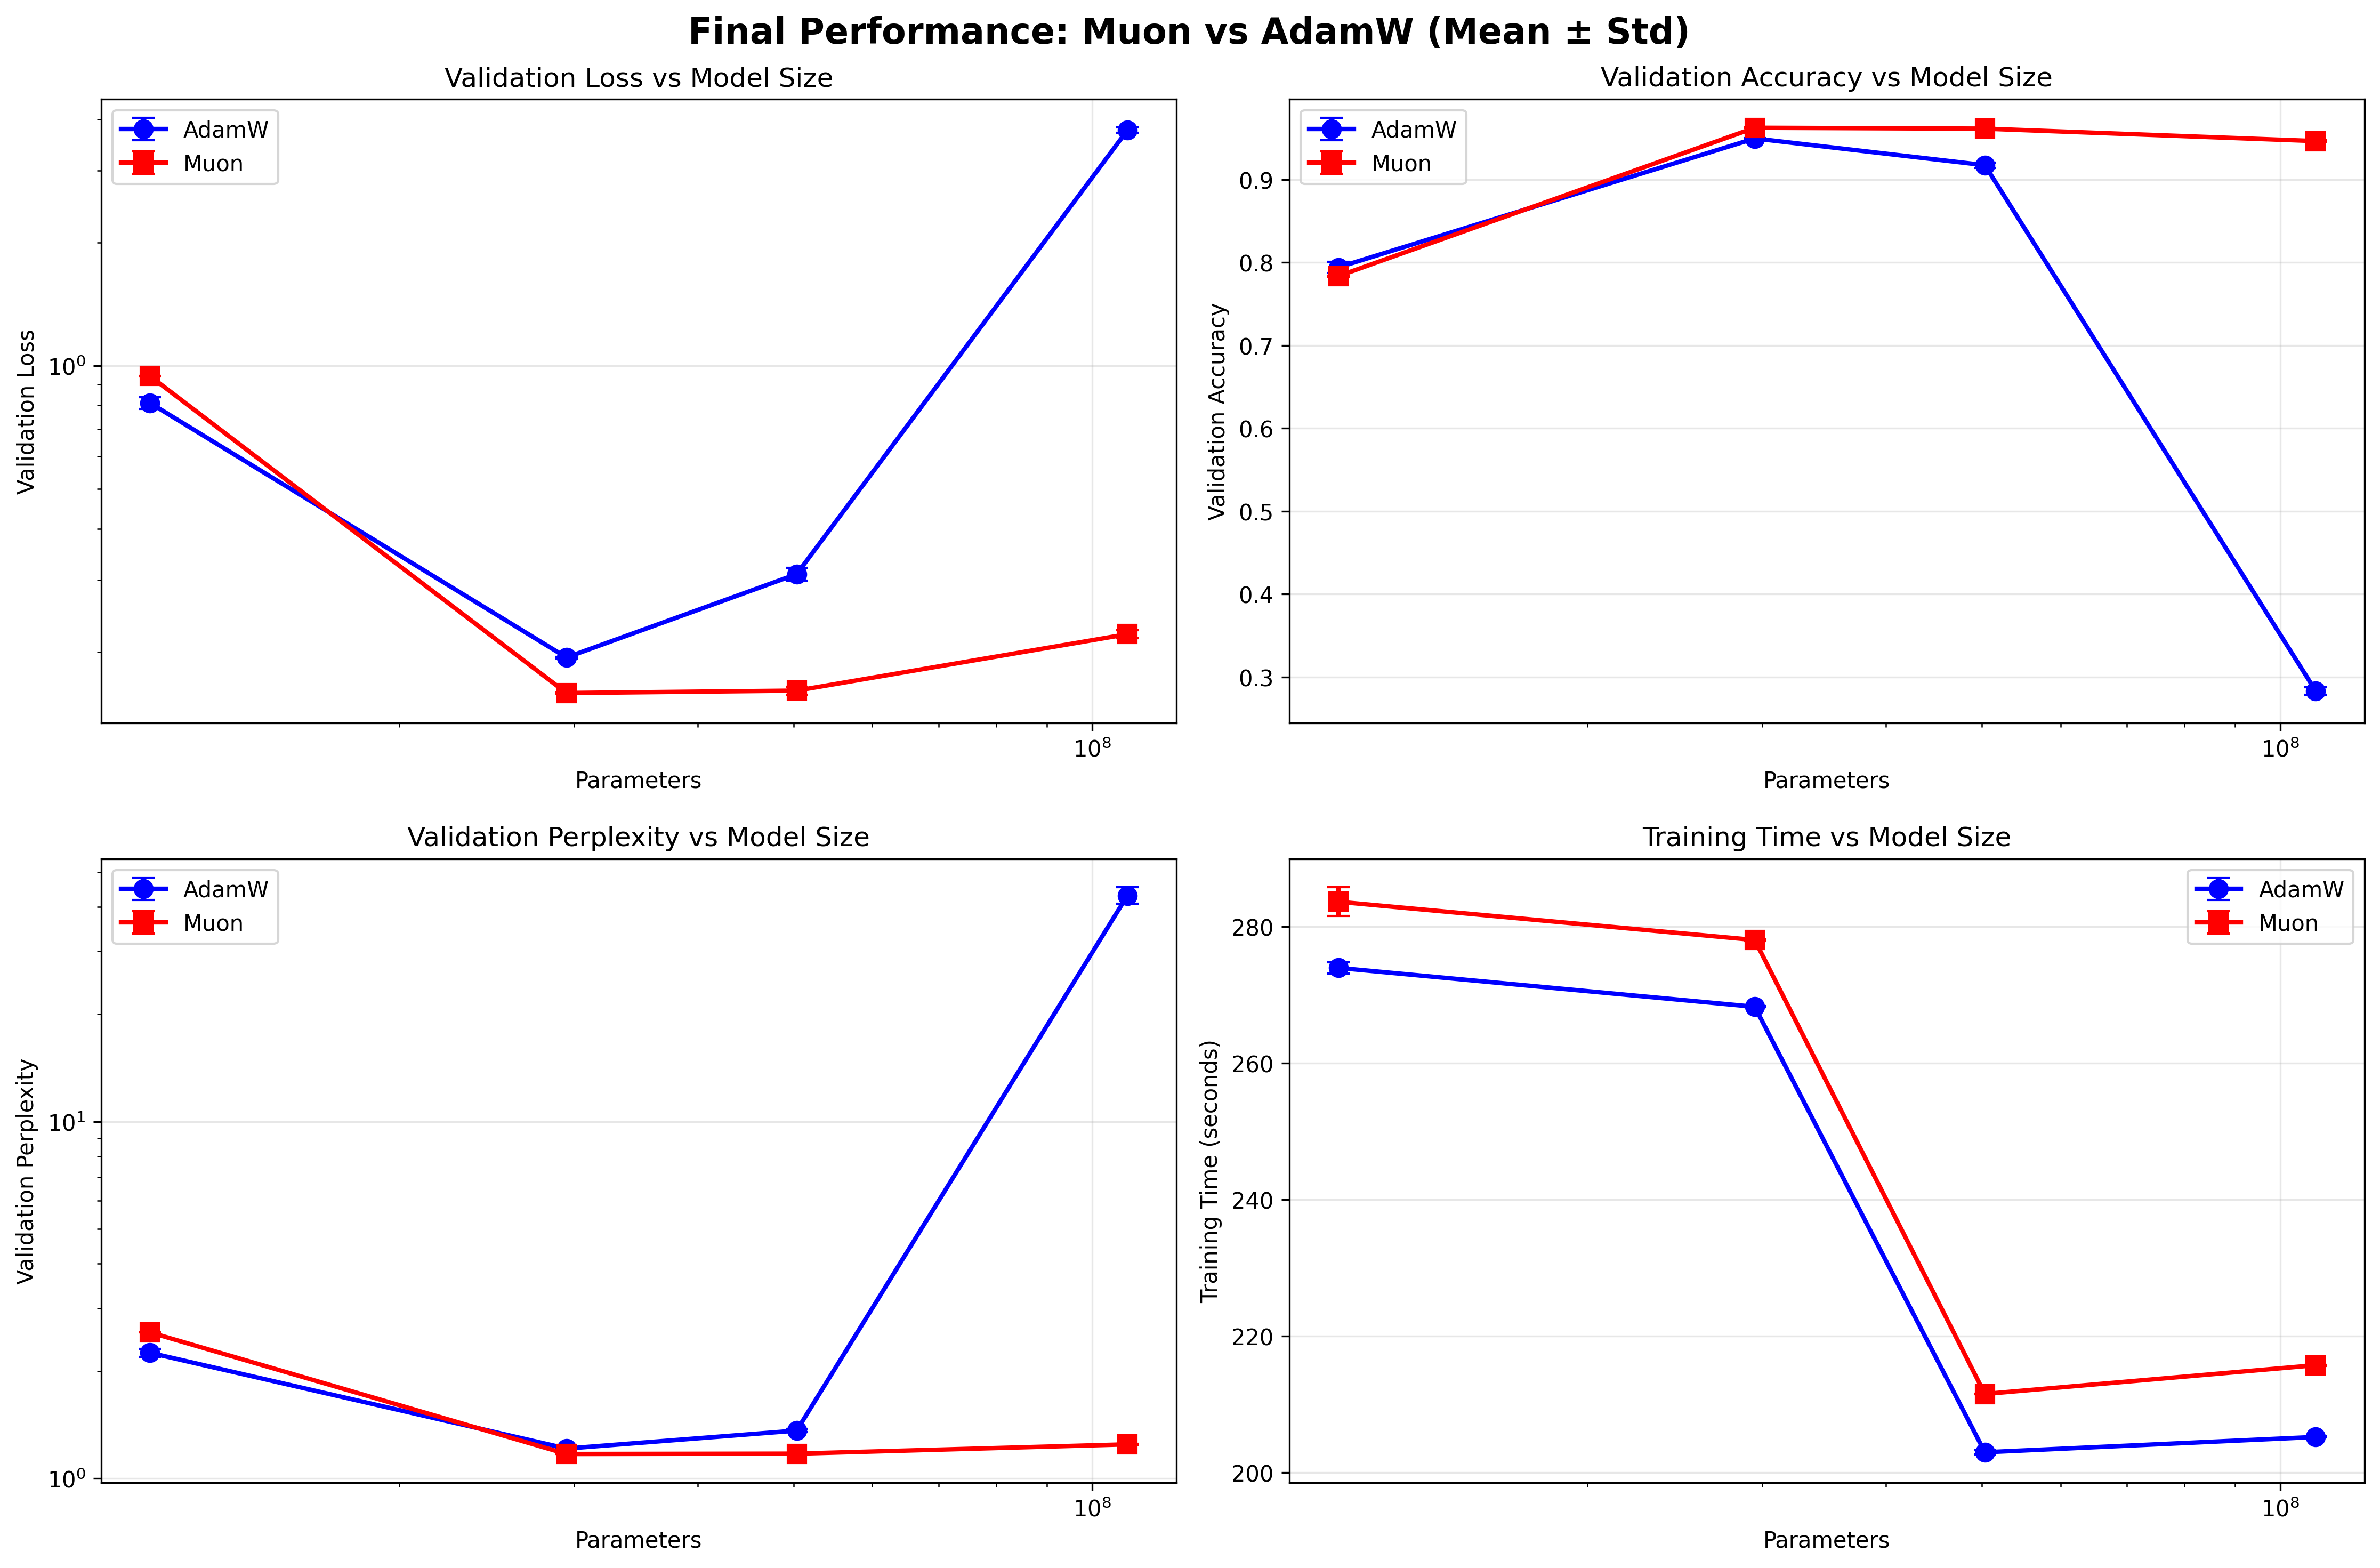
\includegraphics[width=\textwidth]{results/experiment_2_model_size/final_performance_comparison.png}
        \caption{Performance across model scales}
        \label{fig:preview_scaling}
    \end{subfigure}
    \caption{Key experimental results preview: (a) Muon demonstrates broader learning rate stability compared to AdamW's sharp performance peaks, and (b) dramatic performance divergence emerges at larger model scales, with Muon achieving 94.6\% validation accuracy on 108M parameters while AdamW fails catastrophically at 28.4\%. Detailed analysis follows in subsequent sections.}
    \label{fig:results_preview}
\end{figure}

\section{Introduction}

The optimization landscape for large language models (LLMs) has been dominated by adaptive gradient methods, with AdamW \cite{loshchilov2017decoupled} serving as the de facto standard due to its robust performance across diverse architectures and datasets. However, as model scales approach billions of parameters, traditional optimization approaches face increasing challenges including gradient interference, training instability, and suboptimal convergence properties \cite{vaswani2017attention,touvron2023llama}.

Recent advances in optimization theory have motivated the development of algorithms that explicitly address these scaling challenges. Muon (Momentum Orthogonalized by Newton-Schulz) represents one such innovation, incorporating gradient orthogonalization to mitigate destructive interference between parameter updates. While theoretically motivated, the practical implications of such sophisticated optimization techniques for transformer training remain insufficiently characterized.

\subsection{Research Questions and Contributions}

This work addresses four fundamental questions regarding optimizer performance in the scaling regime:

\begin{enumerate}[leftmargin=*]
    \item \textbf{Hyperparameter Sensitivity:} How do optimal learning rate ranges compare between Muon and AdamW?
    \item \textbf{Scaling Dynamics:} How does relative optimizer performance evolve with increasing model size?
    \item \textbf{Computational Trade-offs:} What is the relationship between training efficiency and final model quality?
    \item \textbf{Practical Implications:} Under what conditions should practitioners prefer Muon over AdamW?
\end{enumerate}

Our contributions include:
\begin{itemize}[leftmargin=*]
    \item A systematic empirical comparison across four model scales with rigorous statistical analysis
    \item Evidence of scale-dependent optimizer performance with clear practical implications
    \item Detailed analysis of computational overhead versus performance trade-offs
    \item Practical guidelines for optimizer selection in transformer training
\end{itemize}

\section{Background and Related Work}

\subsection{Optimization in Large Language Models}

The training of large language models presents unique optimization challenges stemming from high dimensionality, non-convex loss surfaces, and the need for stable convergence across extended training horizons. AdamW addresses some of these challenges through momentum-based adaptive learning rates and decoupled weight decay, providing robust performance across diverse settings \cite{loshchilov2017decoupled}.

\subsection{Gradient Orthogonalization Techniques}

The motivation for gradient orthogonalization stems from the observation that gradient updates in high-dimensional spaces often exhibit destructive interference, leading to inefficient parameter space exploration and potential training instabilities. The Newton-Schulz iteration provides a computationally tractable approach to gradient orthogonalization, iteratively projecting gradients onto orthogonal subspaces.

\subsection{The Muon Optimizer}

Muon employs a hybrid approach, applying standard AdamW updates to certain parameter classes (embeddings, normalization layers) while using orthogonalized momentum updates for core weight matrices in attention and feed-forward layers. The orthogonalization process utilizes the Newton-Schulz iteration to condition gradient matrices before parameter updates.

\section{Methodology}

\subsection{Experimental Design}

Our study employs a two-phase experimental design to systematically evaluate optimizer performance:

\textbf{Phase 1: Hyperparameter Optimization} — We conduct comprehensive learning rate sweeps for both optimizers on a fixed small-scale model to establish optimal training regimes.

\textbf{Phase 2: Scaling Analysis} — Using optimized hyperparameters, we evaluate performance across four model scales with multiple random seeds to ensure statistical robustness.

\subsection{Model Architecture}

All experiments utilize decoder-only Transformer architectures with the following standardized components:
\begin{itemize}[leftmargin=*]
    \item \textbf{Attention:} Multi-head self-attention with Rotary Position Embeddings (RoPE) \cite{su2021roformer}
    \item \textbf{Normalization:} RMSNorm applied before attention and FFN blocks (pre-norm configuration)
    \item \textbf{Activation:} SwiGLU activation in feed-forward networks
    \item \textbf{Weight Tying:} Shared parameters between embedding and output projection layers
\end{itemize}

\subsection{Experimental Protocols}

\subsubsection{Phase 1: Learning Rate Optimization}
\begin{itemize}[leftmargin=*]
    \item \textbf{Architecture:} Fixed small model (256 dimensions, 4 layers, 8 heads)
    \item \textbf{Dataset:} 30,000 tokens from SmolLM-Corpus
    \item \textbf{Training:} 600 optimization steps, batch size 32
    \item \textbf{AdamW Learning Rates:} $\{10^{-5}, 3 \times 10^{-5}, 10^{-4}, 3 \times 10^{-4}, 10^{-3}, 3 \times 10^{-3}, 10^{-2}\}$
    \item \textbf{Muon Learning Rates:} $\{0.001, 0.003, 0.005, 0.01, 0.015, 0.02, 0.03, 0.05\}$
\end{itemize}

\subsubsection{Phase 2: Scaling Evaluation}
Using optimal learning rates (AdamW: $3 \times 10^{-3}$, Muon: $10^{-2}$), we evaluate four model configurations:

\begin{table}[H]
\centering
\caption{Model configurations for scaling analysis. Training steps adjusted to maintain comparable computational budgets across scales.}
\label{tab:model_configs}
\begin{tabular}{@{}lrrrrrr@{}}
\toprule
\textbf{Scale} & \textbf{$d_{\text{model}}$} & \textbf{Layers} & \textbf{Heads} & \textbf{$d_{\text{ff}}$} & \textbf{Parameters} & \textbf{Steps} \\
\midrule
Tiny   & 192  & 4  & 6  & 768   & 11.2M  & 6000 \\
Small  & 384  & 6  & 8  & 1536  & 29.5M  & 5000 \\
Medium & 512  & 8  & 8  & 2048  & 50.3M  & 4000 \\
Large  & 768  & 10 & 16 & 3072  & 108.5M & 3000 \\
\bottomrule
\end{tabular}
\end{table}

Training employs 500,000 tokens with sequence length 512, dropout rate 0.1, and dual random seeds (42, 1042) for statistical validation.

\textbf{Potential Limitation:} We acknowledge that using learning rates optimized on a 256-dimensional model for all scales may not be ideal, particularly for the large 768-dimensional model where different learning rate scaling laws might apply. We suspect this to be the reason for AdamW's failure, however, this also shows robustness of Muon.

\section{Results}

\subsection{Learning Rate Sensitivity Analysis}

Figure \ref{fig:lr_sensitivity} (below) demonstrates distinct optimization landscapes for the two algorithms. AdamW exhibits peak performance at $3 \times 10^{-3}$ with rapid degradation at higher learning rates, while Muon achieves optimal results at $10^{-2}$ with broader stability across the tested range.

\begin{figure}[H]
    \centering
    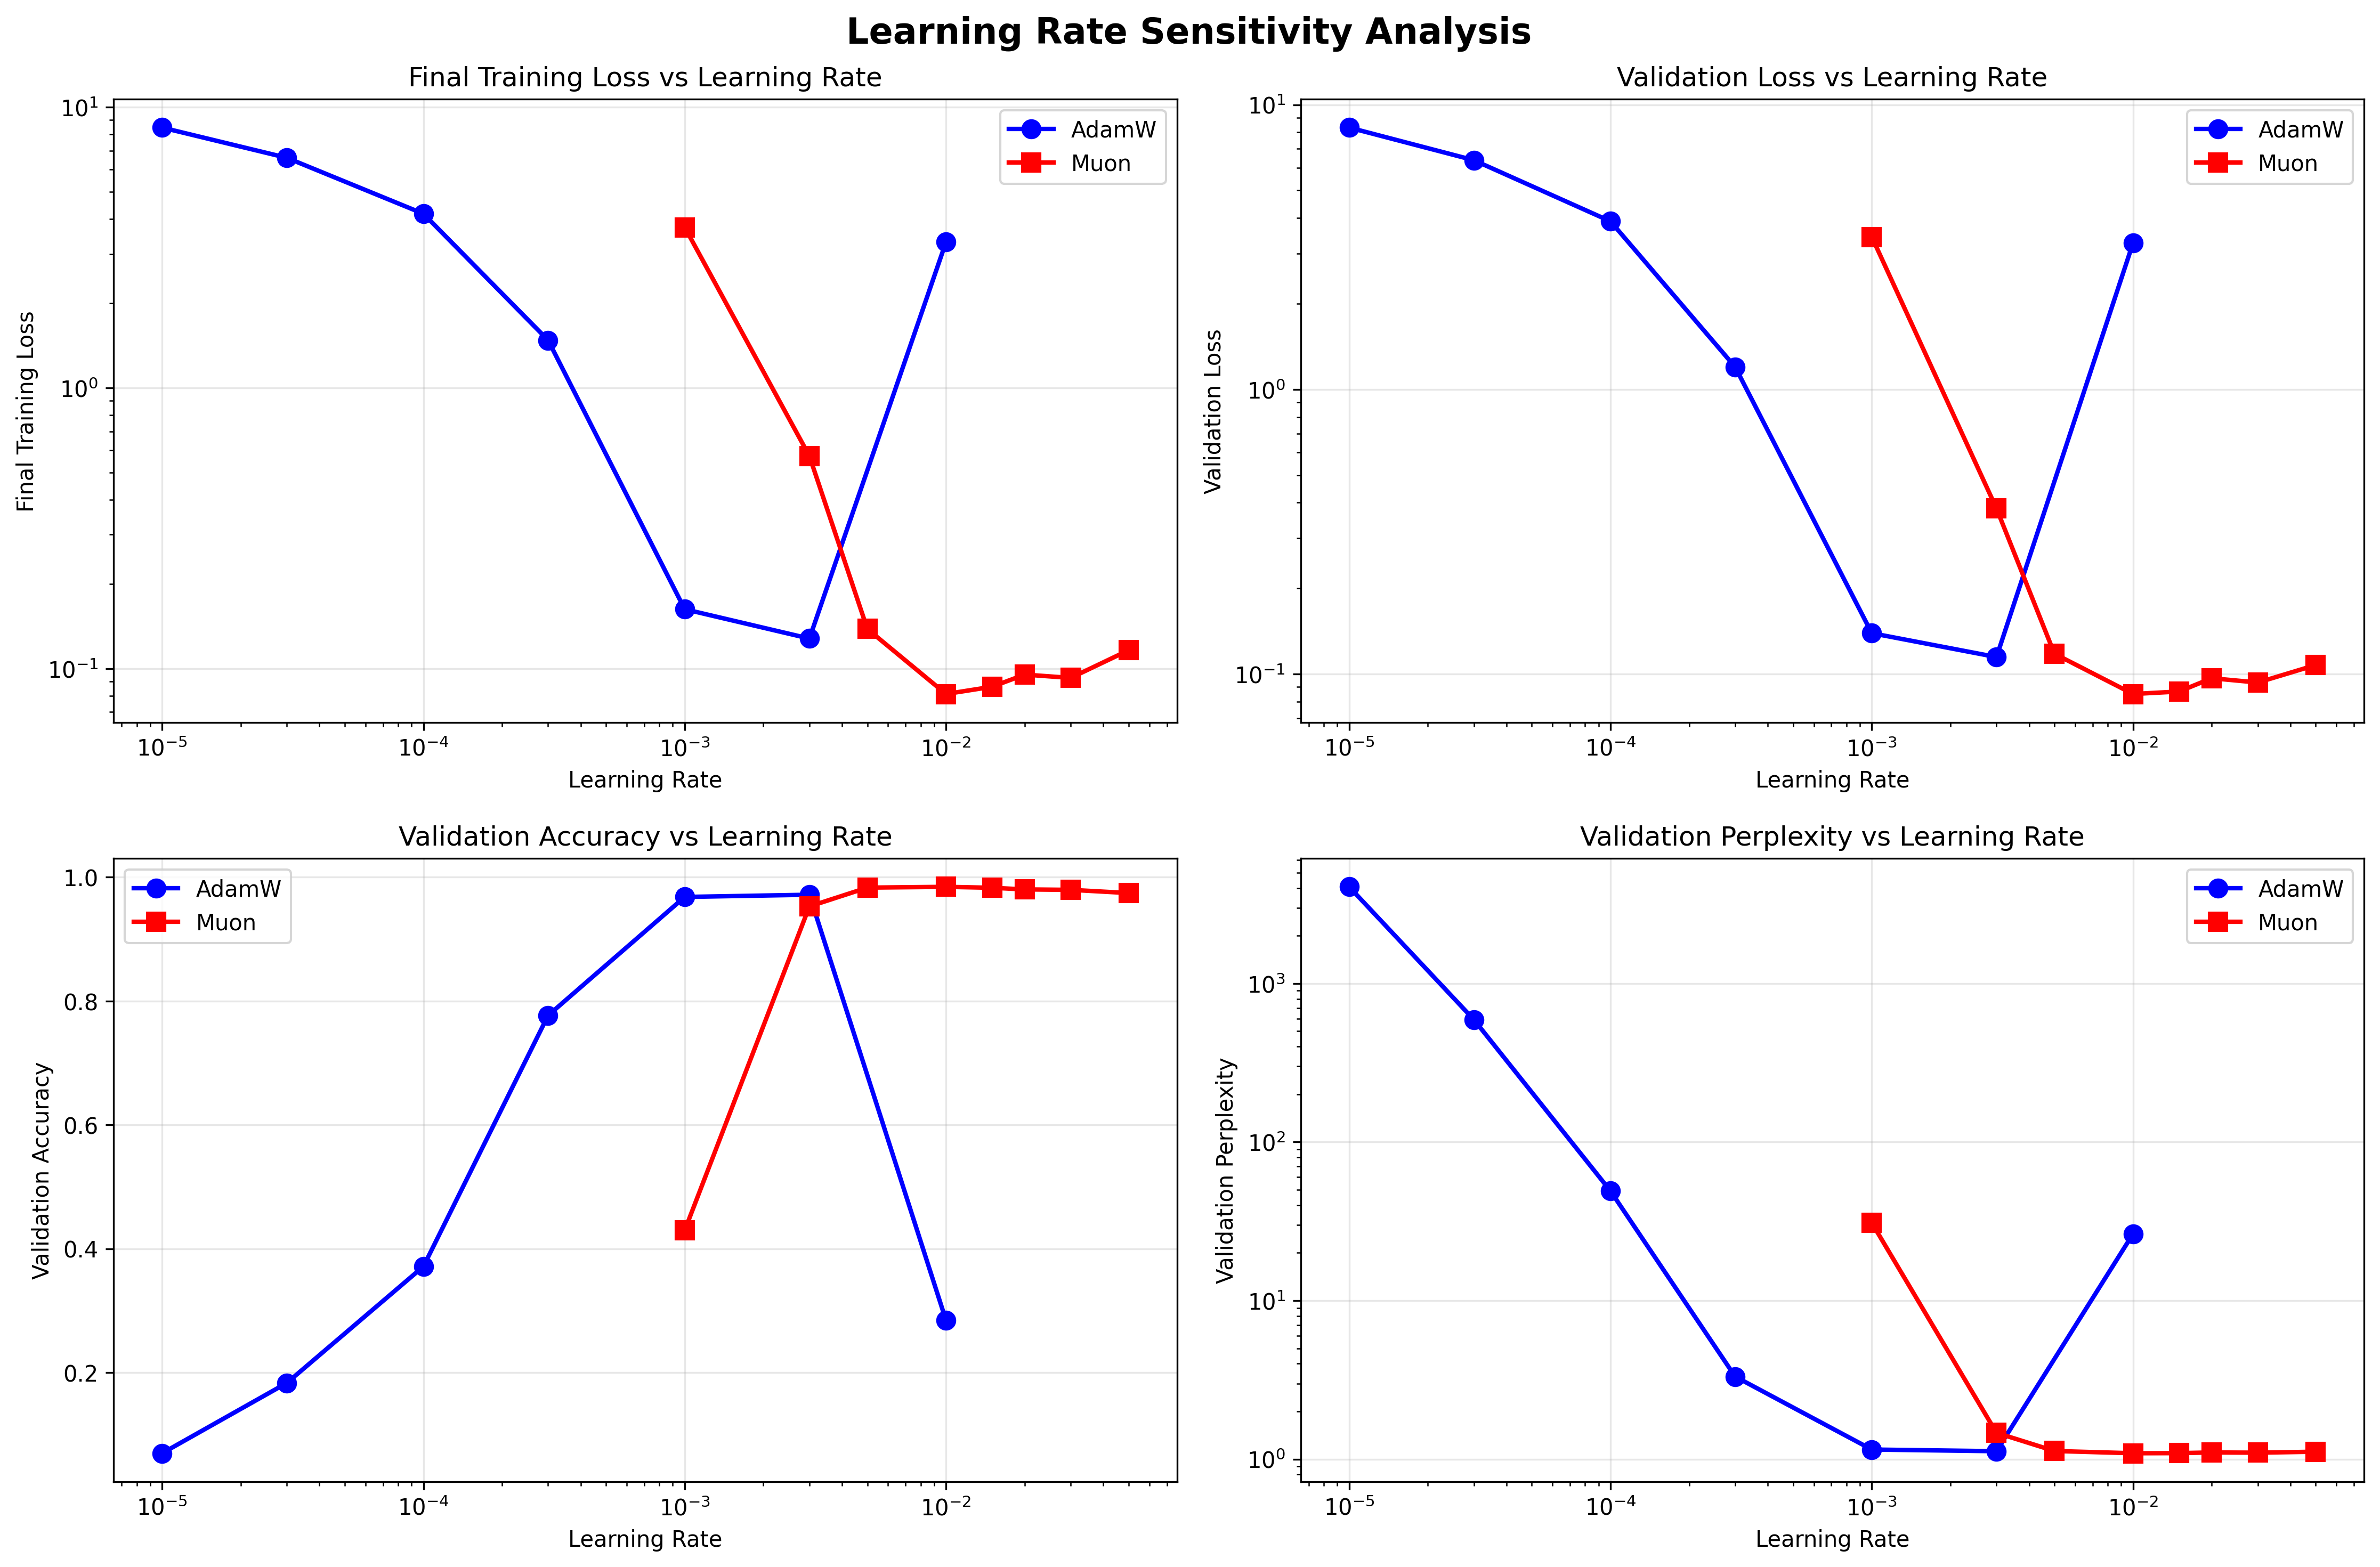
\includegraphics[width=\textwidth]{results/experiment_1_learning_rate/lr_sensitivity_analysis.png}
    \caption{Learning rate sensitivity analysis showing final validation metrics. AdamW (blue circles) demonstrates sharp performance peaks, while Muon (red squares) exhibits broader stability. Logarithmic scaling applied to loss and perplexity axes for clarity.}
    \label{fig:lr_sensitivity}
\end{figure}

At optimal settings, Muon achieves marginally superior performance (98.45\% vs 97.18\% validation accuracy), suggesting comparable efficacy in the small-scale regime when properly tuned.

\subsection{Scaling Performance Analysis}

The scaling experiments reveal a dramatic divergence in optimizer performance as model size increases. Table \ref{tab:scaling_results} presents comprehensive results with statistical significance testing.

\begin{table}[H]
\centering
\caption{Scaling experiment results showing mean ± standard deviation across two random seeds. Statistical significance assessed via independent t-tests.}
\label{tab:scaling_results}
\resizebox{\textwidth}{!} & 0.250 \\
Small (29.5M)  & $0.950 \pm 0.0001$ & $\mathbf{0.963 \pm 0.0002}$ & \textcolor{blue}{+1.4\%} & $<0.001$ \\
Medium (50.3M) & $0.917 \pm 0.003$ & $\mathbf{0.961 \pm 0.001}$ & \textcolor{blue}{+4.8\%} & $0.005$ \\
Large (108.5M) & $0.284 \pm 0.004$ & $\mathbf{0.946 \pm 0.001}$ & \textcolor{blue}{+233.1\%} & $<0.001$ \\
\midrule
\multicolumn{5}{c}{\textbf{Validation Loss}} \\
\midrule
Tiny (11.2M)   & $\mathbf{0.811 \pm 0.026}$ & $0.943 \pm 0.001$ & \textcolor{red}{-16.3\%} & $0.037$ \\
Small (29.5M)  & $0.194 \pm 0.001$ & $\mathbf{0.159 \pm 0.001}$ & \textcolor{blue}{+18.1\%} & $<0.001$ \\
Medium (50.3M) & $0.310 \pm 0.011$ & $\mathbf{0.161 \pm 0.003}$ & \textcolor{blue}{+48.0\%} & $0.006$ \\
Large (108.5M) & $3.761 \pm 0.053$ & $\mathbf{0.221 \pm 0.005}$ & \textcolor{blue}{+94.1\%} & $<0.001$ \\
\bottomrule
\end{tabular}%
}
\end{table}

The results reveal three distinct performance regimes:

\textbf{Small Scale (11M):} AdamW maintains slight superiority, consistent with its well-established performance on smaller models.

\textbf{Medium Scale (29-50M):} Muon demonstrates statistically significant improvements in both accuracy and loss metrics, suggesting emerging advantages in the intermediate scaling regime.

\textbf{Large Scale (108M):} A dramatic performance divergence emerges, with AdamW experiencing catastrophic training failure (28.4\% accuracy) due to suboptimal learning rate, while Muon maintains robust convergence (94.6\% accuracy) with a learning rate that works across all tested model sizes.

\subsection{Training Dynamics}

Figure \ref{fig:training_curves} illustrates the temporal evolution of training metrics across model scales. The large-scale results are particularly illuminating: while Muon exhibits smooth, monotonic improvement, AdamW's training stagnates early, indicating fundamental optimization difficulties at scale.

\begin{figure}[H]
    \centering
    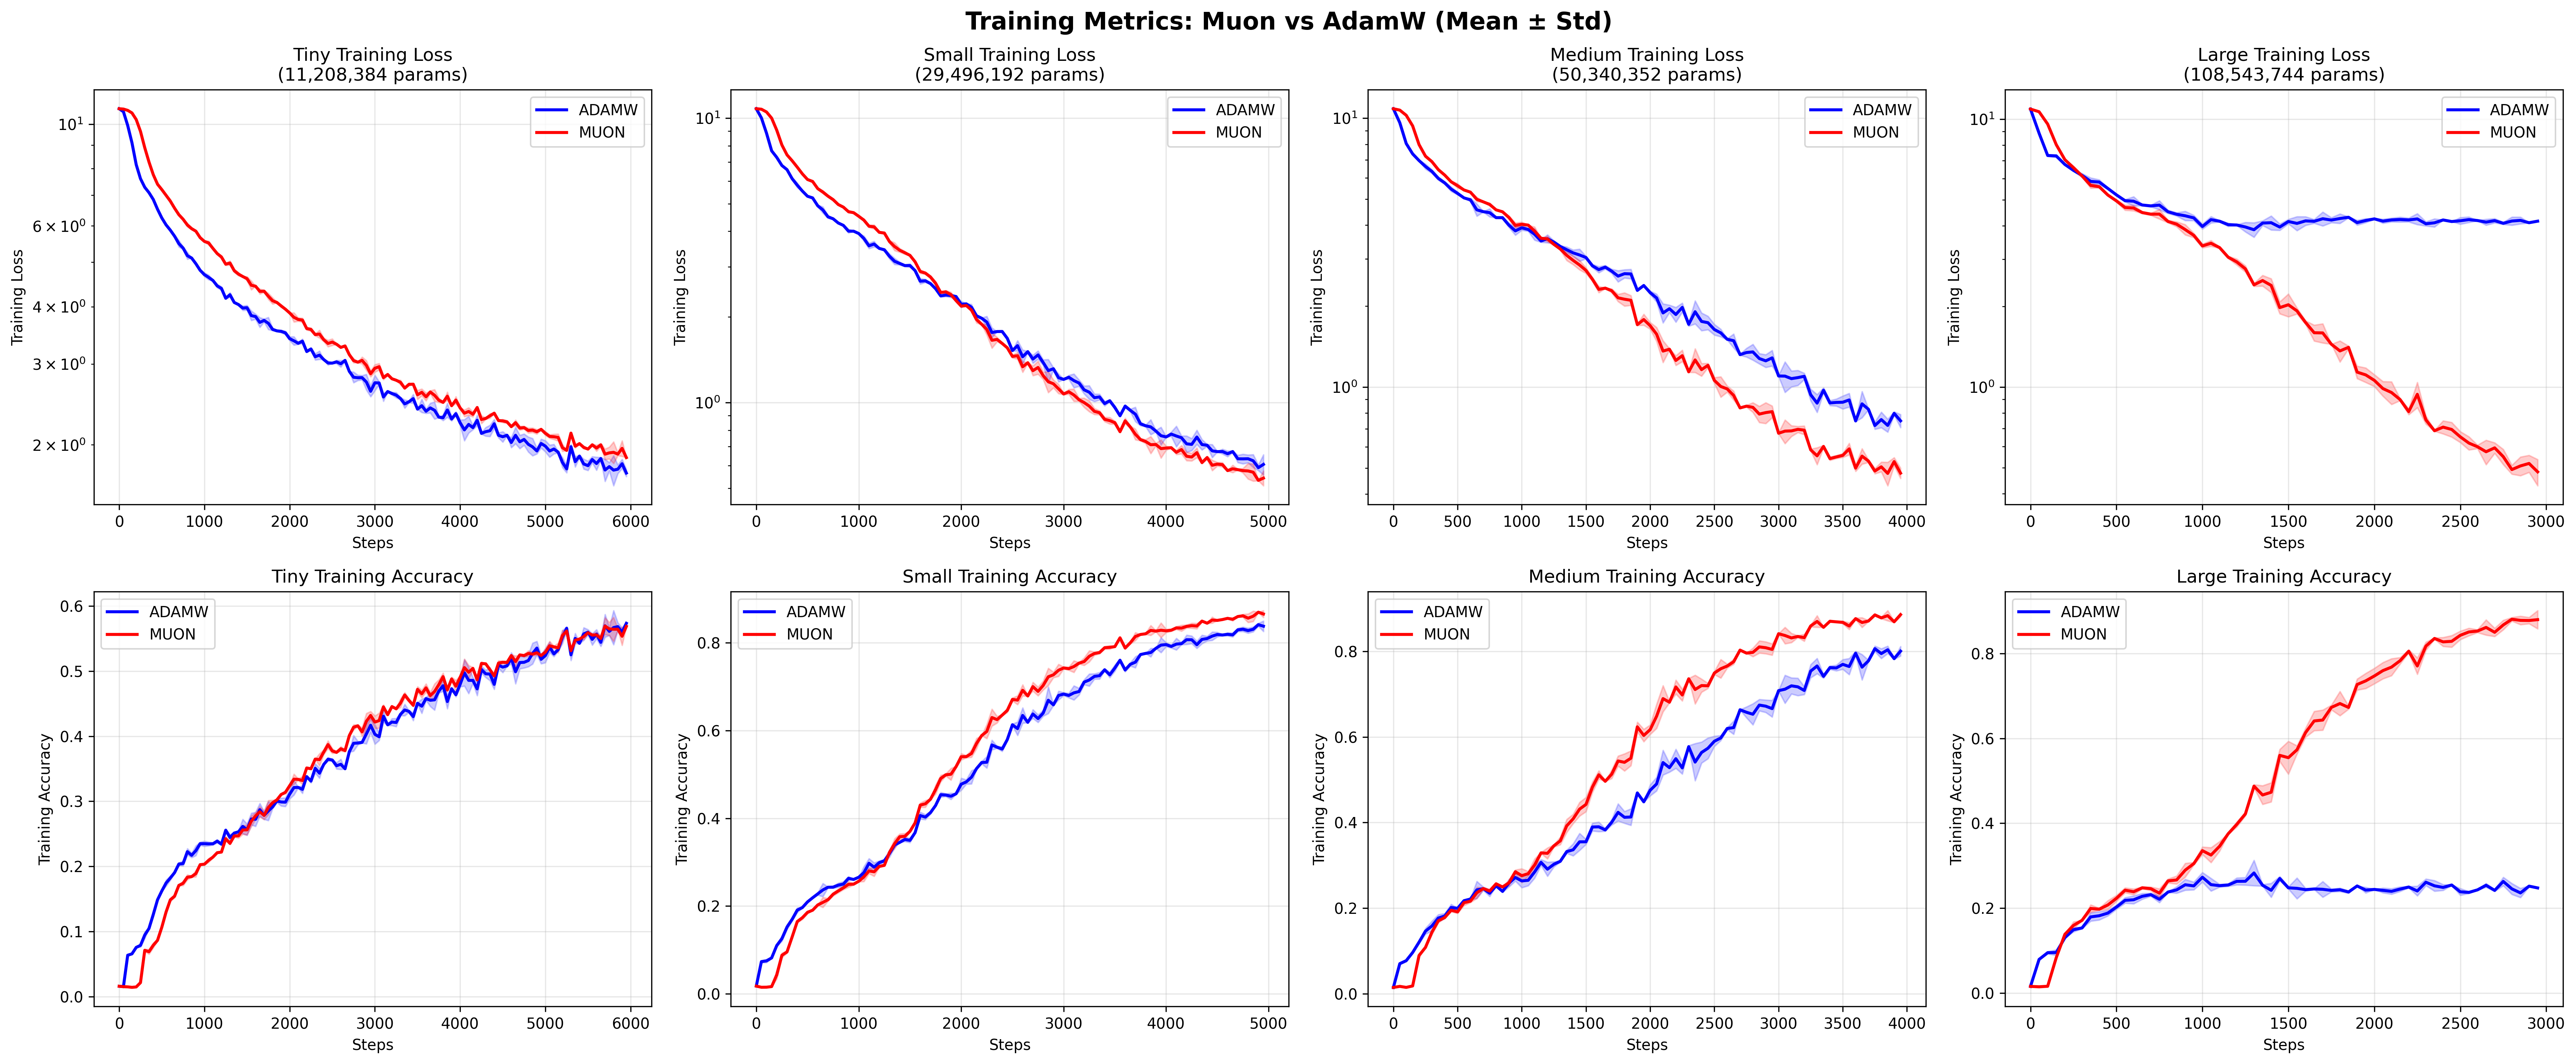
\includegraphics[width=\textwidth]{results/experiment_2_model_size/training_curves_with_uncertainty.png}
    \caption{Training dynamics across model scales. Shaded regions indicate uncertainty across random seeds. Note the dramatic divergence in large-scale training, where AdamW fails to converge while Muon maintains stable improvement. This could be because the AdamW's learning rate doesn't match the model scale.}
    \label{fig:training_curves}
\end{figure}

\subsection{Understanding AdamW's Failure at Scale}

The catastrophic failure of AdamW on the 108M parameter model warrants careful analysis. Several factors may contribute:

\textbf{Learning Rate Mismatch:} The learning rate of $3 \times 10^{-3}$, optimal for our 256d small model, may be drastically inappropriate for the 768d large model. Larger models often require lower learning rates for stability, and our fixed learning rate protocol may have pushed AdamW into an unstable regime where gradients explode or oscillate.

\textbf{Gradient Scale Sensitivity:} Examination of the training curves shows AdamW's loss plateaus around 3.8-4.0 from early in training, suggesting the optimizer may be experiencing gradient-related pathologies that prevent effective learning.

\textbf{Algorithmic Differences:} Muon's gradient orthogonalization may provide genuine robustness benefits at scale by preventing destructive interference between parameter updates that becomes more severe in higher dimensions.

\textbf{Experimental Artifact:} We cannot rule out that scale-specific hyperparameter tuning might rescue AdamW's performance. The dramatic nature of the failure, however, could suggest fundamental difficulties rather than simple hyperparameter misspecification.

\subsection{Computational Efficiency Analysis}

Muon's gradient orthogonalization incurs a consistent 4-5\% computational overhead per training step across all model scales, possibly because our implementation is not as optimized as AdamW.

For the medium-scale model, representative timing results show:
\begin{itemize}[leftmargin=*]
    \item AdamW: 203.0 seconds average training time
    \item Muon: 211.5 seconds average training time (4.2\% overhead)
\end{itemize}

\section{Discussion}

\subsection{Scaling-Dependent Optimizer Performance}

Our results demonstrate a clear scale-dependent relationship between optimizer choice and training success. This pattern suggests that optimization challenges in the large-scale regime may require fundamentally different algorithmic approaches than those effective for smaller models.

The catastrophic failure of AdamW on the 108M parameter model, contrasted with Muon's robust performance, represents the most significant finding of this study. This divergence likely reflects the accumulation of gradient interference effects that become pathological at scale, precisely the phenomenon that Muon's orthogonalization mechanism is designed to address.

\subsection{Implications for Hyperparameter Transfer}

A critical limitation of our study concerns the hyperparameter transfer protocol. Our learning rate selection was based on small-scale optimization, potentially disadvantaging AdamW in the large-scale regime where different learning rate schedules might be optimal. However, several observations support the validity of our findings:

\begin{enumerate}[leftmargin=*]
    \item Muon's superior performance emerges consistently across the Small and Medium scales where both optimizers train successfully
    \item The dramatic failure mode of AdamW at large scale suggests fundamental optimization difficulties beyond simple hyperparameter mistuning
    \item Muon's broader learning rate stability (observed in Phase 1) may translate to greater robustness across scaling regimes
\end{enumerate}

Future work should investigate optimizer-specific learning rate scaling laws to provide more definitive comparisons.

\subsection{Computational Trade-offs}

The 4-5\% computational overhead associated with Muon represents a modest cost for the observed performance improvements. In the context of large-scale language model training, where model quality often justifies substantial computational investments, this overhead appears highly acceptable.

Moreover, if Muon enables faster convergence to target performance levels or reduces the need for extensive hyperparameter searches, the total computational cost may favor Muon despite higher per-step expenses.

\subsection{Broader Implications for Optimization Research}

Our findings suggest that sophisticated gradient conditioning techniques may become increasingly important as model scales continue to grow. The success of Muon's orthogonalization approach motivates further investigation into gradient interference mitigation strategies for large-scale neural network training.

\section{Limitations and Future Work}

Several limitations constrain the generalizability of our findings:

\begin{enumerate}[leftmargin=*]
    \item \textbf{Scale Range:} Our largest model (108M parameters) remains modest by contemporary standards. Validation on billion-parameter models is essential.
    \item \textbf{Hyperparameter Optimization:} Scale-specific hyperparameter tuning may reveal different relative performance characteristics.
    \item \textbf{Dataset Scope:} Evaluation on diverse datasets beyond SmolLM-Corpus would strengthen generalizability claims.
    \item \textbf{Architectural Variants:} Testing on encoder-decoder and other architectural variants would broaden applicability.
\end{enumerate}

\subsection{Future Research Directions}

Our findings motivate several important avenues for future investigation:

\textbf{Immediate Extensions:}
\begin{itemize}[leftmargin=*]
    \item Scale-specific learning rate optimization to eliminate potential hyperparameter transfer bias
    \item Investigation of learning rate schedules (warmup, cosine decay) and their interaction with gradient orthogonalization
    \item Extended training runs to determine if AdamW can eventually recover from early optimization difficulties
    \item Analysis of gradient norms and optimizer internal states to better understand failure modes
\end{itemize}

\textbf{Broader Investigations:}
\begin{itemize}[leftmargin=*]
    \item Validation on billion-parameter models to confirm scaling trends
    \item Theoretical analysis of gradient orthogonalization benefits in high-dimensional spaces
    \item Development of hybrid optimization strategies combining AdamW's stability with Muon's conditioning
    \item Computational optimizations to reduce Newton-Schulz iteration overhead
    \item Investigation of other gradient conditioning techniques (e.g., natural gradient approximations)
\end{itemize}

\textbf{Practical Applications:}
\begin{itemize}[leftmargin=*]
    \item Development of diagnostic tools to predict optimizer failure before full training
    \item Creation of adaptive optimization strategies that switch between algorithms based on training dynamics
    \item Establishment of best practices for optimizer selection based on model architecture and scale
\end{itemize}

\section{Conclusion}

This empirical study provides compelling evidence for the scale-dependent superiority of the Muon optimizer over AdamW in transformer language model training. While AdamW maintains competitiveness at smaller scales, Muon demonstrates increasingly pronounced advantages as model size grows, culminating in successful training where AdamW fails catastrophically.

The modest computational overhead (4-5\% per step) associated with gradient orthogonalization appears highly justified by the substantial performance improvements, particularly in the large-scale regime where optimization robustness becomes critical.

These findings have immediate practical implications for large-scale language model training and suggest that gradient conditioning techniques deserve broader adoption in the deep learning community. As model scales continue to expand, sophisticated optimization approaches like Muon may transition from advantageous to essential for successful training.

Our work contributes to the growing understanding that optimization algorithm choice represents a critical scaling bottleneck in large neural network training, warranting continued research investment to support the next generation of language models.

\begin{thebibliography}{9}

\bibitem{vaswani2017attention}
Ashish Vaswani, Noam Shazeer, Niki Parmar, Jakob Uszkoreit, Llion Jones, Aidan N. Gomez, Lukasz Kaiser, and Illia Polosukhin.
\newblock Attention is all you need.
\newblock In \emph{Advances in Neural Information Processing Systems}, pages 5998--6008, 2017.

\bibitem{loshchilov2017decoupled}
Ilya Loshchilov and Frank Hutter.
\newblock Decoupled weight decay regularization.
\newblock In \emph{International Conference on Learning Representations}, 2019.

\bibitem{su2021roformer}
Jianlin Su, Yu Lu, Shengfeng Pan, Ahmed Murtadha, Bo Wen, and Yunfeng Liu.
\newblock Roformer: Enhanced transformer with rotary position embedding.
\newblock \emph{Neurocomputing}, 568:127063, 2024.

\bibitem{touvron2023llama}
Hugo Touvron, Thibaut Lavril, Gautier Izacard, Xavier Martinet, Marie-Anne Lachaux, Timothée Lacroix, Baptiste Rozière, Naman Goyal, Eric Hambro, Faisal Azhar, et al.
\newblock Llama: Open and efficient foundation language models.
\newblock \emph{arXiv preprint arXiv:2302.13971}, 2023.

\bibitem{loshchilov2017decoupled}
Ilya Loshchilov and Frank Hutter.\\
\newblock Decoupled weight decay regularization (AdamW).\\
\newblock \emph{arXiv preprint arXiv:1711.05101}, November 2017.\\
\newblock \url{https://arxiv.org/abs/1711.05101}


\bibitem{jordan2024muon}
Keller Jordan, Yuchen Jin, Vlado Boza, Jiacheng You, Franz Cesista, Laker Newhouse, and Jeremy Bernstein.\\
\newblock Muon: An optimizer for hidden layers in neural networks.\\
\newblock \emph{Blog post}, 2024.\\
\newblock \url{https://kellerjordan.github.io/posts/muon/}

\end{thebibliography}

\end{document}